% =====================================================================================
% Revised Sections 5-6 for the CS F317 mid-semester report.
% Requires: \usepackage{booktabs,graphicx,amsmath}. Figures are in artifacts/.
% Every number below is generated by a script in the repo; see results/RESULTS.md.
%
% ALSO CHANGE IN EARLIER SECTIONS (they currently state things the evidence does not support):
%  * Abstract: replace "small neural approximation errors (~0.021) accumulate ... causing policy
%    optimization to freeze" with "we measure how a single cost head errs on unseen layouts".
%    Replace "the policy treats unvisited states with high disagreement as dangerous, preventing
%    collisions" with "we test whether ensemble disagreement flags unvisited hazards".
%  * Sec. 2.1, gap 2: present the b = 0 issue as a hypothesis; note lambda is capped (lambda_max).
%  * Table 1: remove the unmeasured "~1.04x" compute figure; soften "Intractable on CNNs" for CPO;
%    re-check the LAMBDA row (it uses a Bayesian world-model posterior, not a plain 5x ensemble).
%  * Sec. 4: "sigma_c >> 0 in unvisited states" is contradicted by Exp. 2A below; state it as the
%    hypothesis being tested.
% =====================================================================================

\section{Work Completed Before Mid-Semester}

All results in this section were produced on the real \texttt{SafetyPointGoal1-v0} environment
(vector observations, $T = 1000$) by scripts in our repository, which log every number to disk.
They are small CPU-scale studies intended to test the assumptions behind our method, not a
reproduction of SafeDreamer.

\subsection{Testbed on Python 3.12}
The released Safety-Gymnasium package cannot be installed or imported on Python $\geq 3.11$
(the current Google Colab runtime): it pins \texttt{pygame==2.1.0} and \texttt{mujoco==2.3.3},
which have no Python~3.12 wheels, and it declares NumPy arrays as dataclass defaults, which
Python~3.11+ rejects at import time. We wrote a patch (48 fields in 24 files) and a reproducible
install recipe. A check over 3{,}000 steps confirmed that the emitted cost equals 1 exactly
when the agent is inside a hazard.
We collected 60{,}000 transitions over 60 random layouts with a held-action random policy
(2.98\% hazard-contact rate); per-step uniform random actions produced no contacts in 2{,}000 steps.

\subsection{Integration test: a training bug found and fixed}
Our first verification script minimised the actor loss $-\hat J^R + \lambda \hat J^C$ with a single
optimiser over \emph{all} parameters, including the reward and cost predictors. The fastest way to
reduce that loss is for the model to predict large rewards and zero cost, so the model ``cheated''
instead of the policy learning (Colab log: imagined reward $1.3\times10^{5}$, cost $-5.8\times10^{4}$).
We rewrote the loop with three separate updates: the world model and cost ensemble are trained only
on supervised losses from replay data, the actor is trained in imagination with the model frozen, and
$\lambda$ is updated by dual ascent. Table~\ref{tab:integration} and Fig.~\ref{fig:integration}
compare both versions on real data with invariant checks at every iteration.

\begin{table}[h]
\centering
\caption{Integration test on real data ($H{=}15$, $K{=}5$, $\kappa{=}1$, 300 iterations).
Checks: every imagined per-step cost in $[0, 1+0.5\kappa]$, imagined reward below the maximum achievable ($\approx 14.3$), all values finite.}
\label{tab:integration}
\begin{tabular}{lcccc}
\toprule
Training loop & Iterations passing & Max imagined reward & Final imagined cost & Final $\lambda$ \\
\midrule
Original (single optimiser), $b{=}0$ & 3/300 & $9.3\times10^{6}$ & $\approx 0$ & 2.65 \\
Fixed, $b{=}0$ & 300/300 & 0.63 & 0.44 & 15.0 \\
Fixed, $b{=}25$ & 150/150 & 0.63 & 0.66 & 0.00 \\
\bottomrule
\end{tabular}
\end{table}

With $b{=}0$, $\lambda$ increases steadily because the estimated cost is never exactly zero, while with
$b{=}25$ it returns to zero (Fig.~\ref{fig:integration}c). This illustrates the pressure a zero
budget puts on $\lambda$; in our implementation $\lambda$ is capped at $\lambda_{\max}=50$.

\begin{figure}[h]
\centering
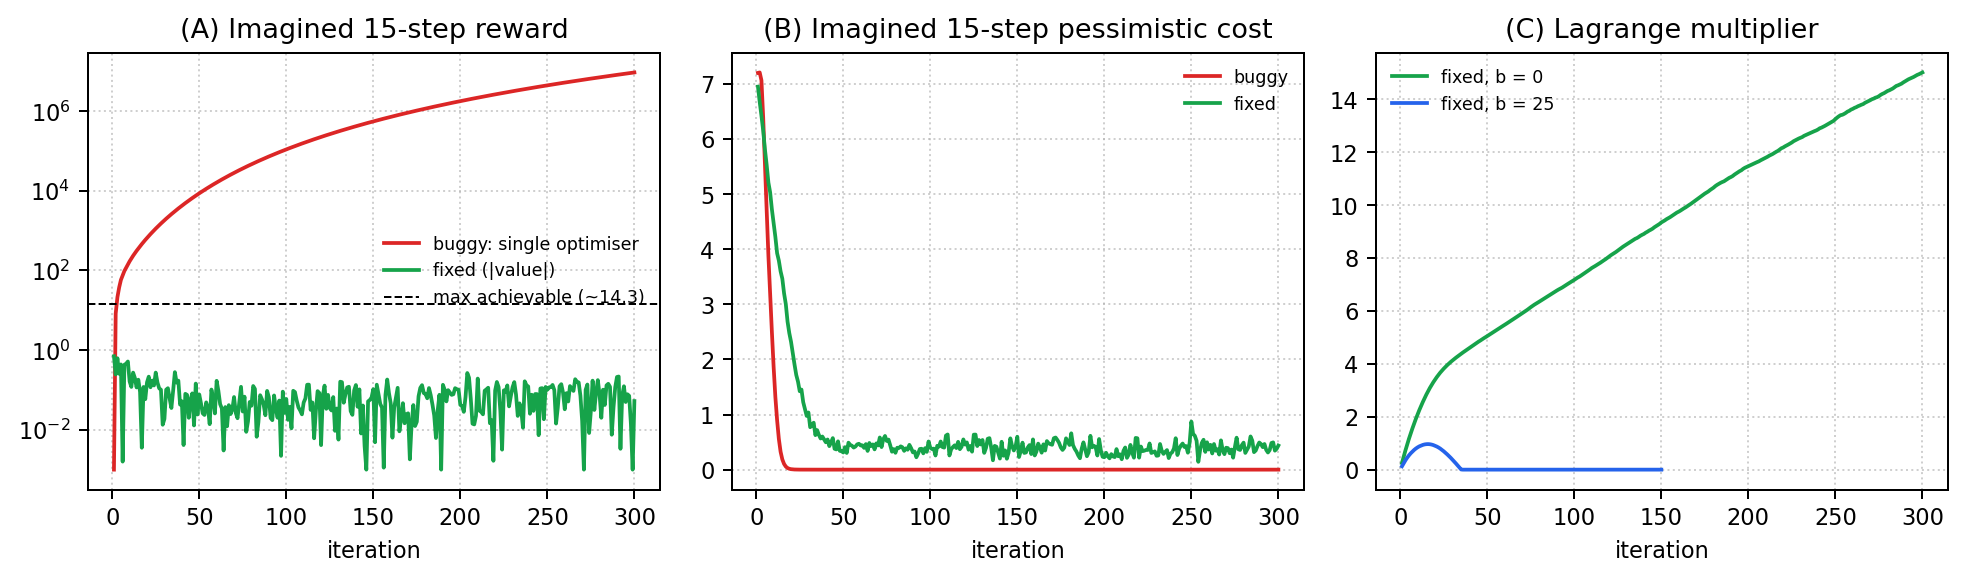
\includegraphics[width=\linewidth]{artifacts/fig_integration_test.png}
\caption{(a) The original loop's imagined reward diverges; the fixed loop stays bounded.
(b) Imagined pessimistic cost. (c) Lagrange multiplier at $b{=}0$ and $b{=}25$.}
\label{fig:integration}
\end{figure}

\subsection{Experiment 1: how a single cost head errs on unseen layouts}
Our draft assumed a single cost head outputs a uniform noise floor of $\hat c \approx 0.021$ in
safe states. We measured this directly: a single head (2$\times$256 MLP) trained on 48 layouts and
tested on 12 held-out layouts, 3 seeds (Table~\ref{tab:exp1}).

\begin{table}[h]
\centering
\caption{Single cost head on held-out layouts (mean $\pm$ std over 3 seeds).}
\label{tab:exp1}
\begin{tabular}{lccccc}
\toprule
Head & Mean $\hat c$ (safe) & Median $\hat c$ (safe) & Mean $\hat c$ (in hazard) & AUROC & $\sum_{t<1000}\hat c$ \\
\midrule
Sigmoid + BCE & $0.023\pm0.003$ & 0.000 & $0.067\pm0.040$ & $0.78\pm0.03$ & 22.8 \\
Linear + MSE  & $0.023\pm0.004$ & 0.001 & $0.072\pm0.038$ & $0.57\pm0.06$ & 22.8 \\
\bottomrule
\end{tabular}
\end{table}

The mean is close to our assumed value, but the mechanism is different. The median prediction in safe
states is essentially zero; the mean is driven by a minority of confident false alarms, and true hazard
states receive low predictions (Fig.~\ref{fig:exp1}). The head reaches AUROC $1.0$ on its training
layouts but $0.78$ on new ones, although the maximum of the hazard-lidar readings alone separates
contacts perfectly. The dominant problem is therefore \emph{generalisation to unseen layouts},
not small regression noise. Summed over the $H{=}15$ imagined horizon the bias is $\approx 0.34$, and as a
discounted return ($\gamma{=}0.99$) it is $\approx 2.3$.

\begin{figure}[h]
\centering
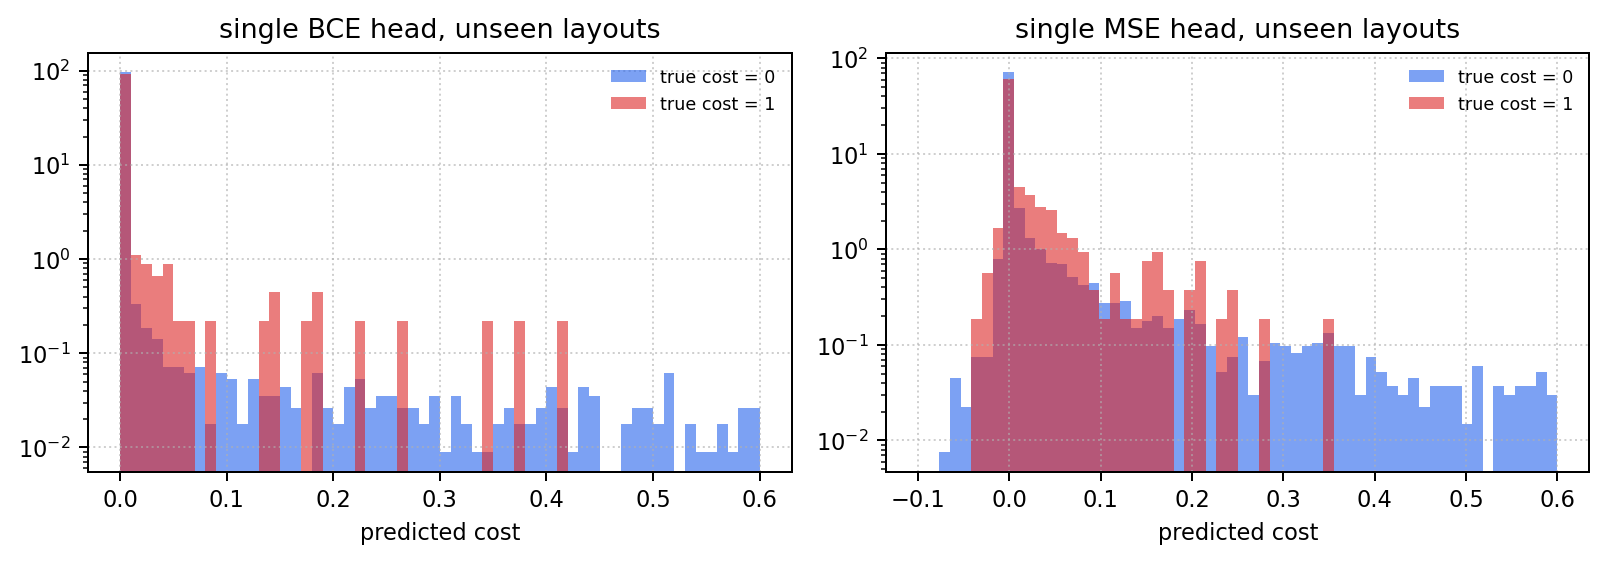
\includegraphics[width=\linewidth]{artifacts/fig_exp1_noise_floor.png}
\caption{Predicted cost on held-out layouts for truly safe and truly hazardous states (log density).}
\label{fig:exp1}
\end{figure}

\subsection{Experiment 2: does ensemble disagreement flag hazards?}
\paragraph{(A) Hazards never seen in training.} We trained the 5-head ensemble only on states farther
than 0.25 from every hazard (42k states, no contacts) and tested on 458 real contacts in held-out
layouts, comparing three variants: random initialisation only, Poisson bootstrap, and bootstrap with
randomised prior functions (Table~\ref{tab:exp2a}).

\begin{table}[h]
\centering
\caption{AUROC for separating real contacts from familiar states (3 seeds; 0.5 = chance).}
\label{tab:exp2a}
\begin{tabular}{lccccc}
\toprule
Variant & $\mu_c$ & $\sigma_c$ & $\mu_c+\sigma_c$ (our method) & $\sigma$ of logits & logit mean $+\,\sigma$ \\
\midrule
Plain      & $0.28\pm0.04$ & $0.32\pm0.03$ & $0.30\pm0.04$ & $0.73\pm0.02$ & $0.30\pm0.04$ \\
Bootstrap  & $0.28\pm0.04$ & $0.30\pm0.03$ & $0.29\pm0.04$ & $0.66\pm0.13$ & $0.29\pm0.04$ \\
Boot+prior & $0.28\pm0.04$ & $0.30\pm0.02$ & $0.29\pm0.04$ & $0.66\pm0.13$ & $0.29\pm0.04$ \\
\bottomrule
\end{tabular}
\end{table}

This contradicts the assumption in Section~4. All heads saturate at ``safe'', so $\sigma_c$ in
probability space is $\approx 3\times10^{-7}$ at contacts, and the pessimistic cost
$\tilde c=\mu_c+\kappa\sigma_c$ is \emph{worse than chance} (it catches 1--2\% of contacts at a 1\%
false-alarm rate). The mean extrapolates in the unsafe direction: predicted cost falls as the agent
approaches a hazard (AUROC 0.28). Disagreement does exist in logit space (AUROC 0.66--0.73), but adding
it to the confidently wrong mean, even before the sigmoid, does not recover the signal.

\paragraph{(B) Data scarcity.} Training on the first $N$ transitions (2 seeds), hazard-detection AUROC
on unseen layouts rises with data ($0.42, 0.52, 0.75, 0.77$ for $N = 1\text{k}, 5\text{k}, 20\text{k}, 48\text{k}$),
while $\kappa \in \{0, 1, 2\}$ changes AUROC by at most $0.003$. However, for $N \geq 20\text{k}$ the
disagreement $\sigma_c$ predicts \emph{where the mean prediction is wrong} with AUROC 0.80--0.86
(Fig.~\ref{fig:exp2}b). Disagreement is therefore informative about model error, but adding it to the
cost does not improve hazard detection.

\begin{figure}[h]
\centering
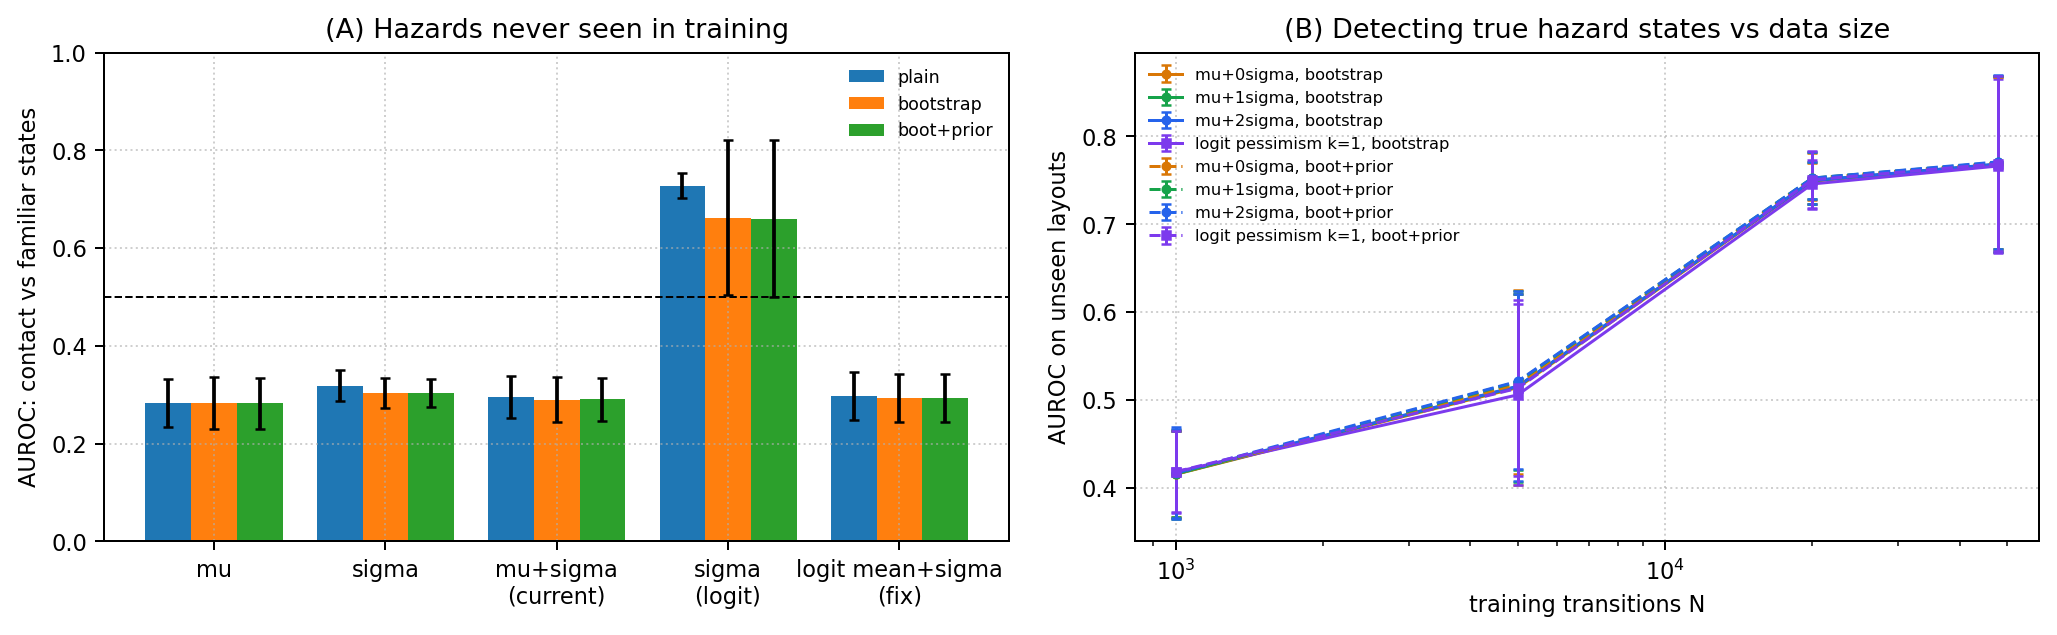
\includegraphics[width=\linewidth]{artifacts/fig_exp2_uncertainty.png}
\caption{(a) Exp.~2A, hazards never seen in training. (b) Exp.~2B, hazard detection versus training data size.}
\label{fig:exp2}
\end{figure}

\subsection{Online pilot}
As an end-to-end sanity check we trained a small deterministic latent world model with the cost
ensemble online (5k random prefill steps, 30k steps total, $b{=}25$, 2 seeds per $\kappa$), together
with a compact PPO-Lagrangian baseline (Table~\ref{tab:pilot}, Fig.~\ref{fig:pilot}).

\begin{table}[h]
\centering
\caption{Online pilot in the real environment. Evaluation: deterministic policy on 10 new layouts.}
\label{tab:pilot}
\begin{tabular}{lccc}
\toprule
Method (seed) & Training violations & Eval.\ return & Eval.\ cost / episode \\
\midrule
Model-based, $\kappa{=}0$ (0) & 1058 & $-4.89$ & 16.7 \\
Model-based, $\kappa{=}0$ (1) & 1377 & $-1.45$ & 1.9 \\
Model-based, $\kappa{=}1$ (0) & 1779 & $-1.88$ & 21.8 \\
Model-based, $\kappa{=}1$ (1) & 808  & $+0.76$ & 76.3 \\
PPO-Lag (0), first 30k / 60k steps & 4250 / 6036 & $-2.37$ & 36.2 \\
\bottomrule
\end{tabular}
\end{table}

The two seeds disagree in sign, so this pilot provides \emph{no evidence} that $\kappa{=}1$ reduces
training-time violations, and no agent learned to reach goals reliably within 30k steps. The pilot
confirms that the full pipeline runs end-to-end; it is far too small to compare methods.

\begin{figure}[h]
\centering
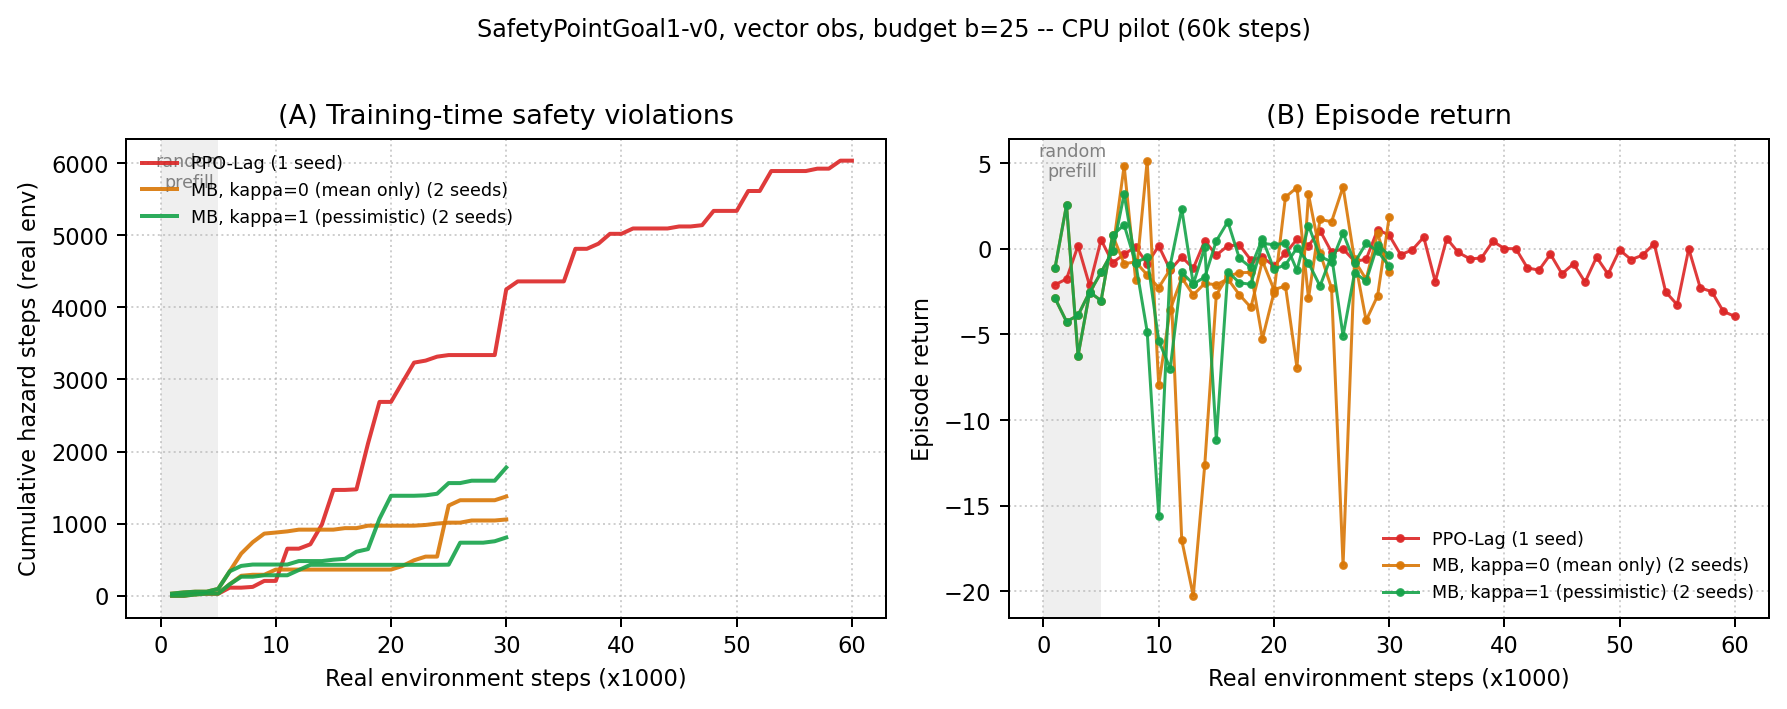
\includegraphics[width=\linewidth]{artifacts/fig_training_curves.png}
\caption{Online pilot: cumulative hazard steps and episode return in the real environment.}
\label{fig:pilot}
\end{figure}

\subsection{Summary of evidence}
Our results support three statements: (i) the corrected training loop is stable and the original
divergence was an optimisation bug; (ii) a single cost head mainly fails by generalising poorly to
unseen layouts; and (iii) ensemble disagreement carries information about model error. They do
\emph{not} yet support the claim that the additive pessimistic cost $\mu_c+\kappa\sigma_c$ flags
unseen hazards or reduces violations. Disagreement in probability space collapses, and the mean
prediction extrapolates in the unsafe direction.

\section{Revised Post-Midsem Plan}
\begin{itemize}
  \item \textbf{Redesign the uncertainty signal.} Use logit-space disagreement as a separate novelty
        penalty with a threshold calibrated on familiar states, and compare it with a dedicated novelty
        detector (e.g.\ random network distillation or latent density), instead of adding $\kappa\sigma_c$ to $\mu_c$.
  \item \textbf{Fix layout generalisation.} Rotation augmentation of the lidar observations; more layouts.
  \item \textbf{Scale the comparison.} Longer runs ($\geq$500k steps) on a Colab GPU with $\geq$3 seeds;
        OmniSafe PPO-Lag and CPO baselines (teammate, Weeks 1--2).
  \item \textbf{Move into SafeDreamer.} Implement the ensemble cost head inside the official (JAX)
        SafeDreamer code for the Stage-3 pixel experiments.
  \item \textbf{Ablations.} $K \in \{1, 3, 5\}$, budget $b \in \{0, 25\}$, and the novelty threshold.
\end{itemize}
